%!TEX root = ../talk.tex

\section{Caffe}\label{sec:Caffe}

%%%

\frameinlbffalse

{
\usebackgroundtemplate{
\tikz[overlay,remember picture] \node[opacity=0.8, xshift=-3cm, at=(current page.east)] {
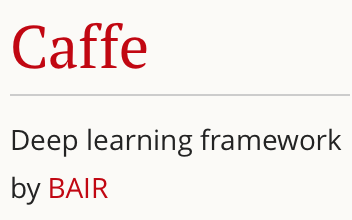
\includegraphics[width=0.3\paperwidth]{figures/Caffe_logo.png}
};}

\begin{frame}[plain]
\frametitle{\S\ref{sec:Caffe}. \insertsection}
\listofframes
\end{frame}
\addtocounter{framenumber}{-1} % this page does not count

}

\frameinlbftrue

%%%
\subsection{Programming interface}
%%%

\begin{frame}
  \MyLogo
  \frametitle{Programming Interface}  

\begin{enumerate}
\item Mainly focus on (and well suited for) CNN and image recognition 
\item Not well documented
\item Expressive architecture 
\begin{itemize}
\item Define models and optimization by configuration without hard-coding
\item With protocol tool to define parameters for nets and solvers $\ldots$
\end{itemize}
\end{enumerate}
\end{frame}

%%%
\subsection{Simple examples}
%%%
\begin{frame}[fragile]
  \MyLogo
  \frametitle{Example: Image Classification}  

\begin{lstlisting}[language=python]
import caffe
import matplotlib.pyplot as plt

# paste your image URL here
my_image_url = "https://wikipedia/Orang_Utan/2C_Malaysia.JPG"
!wget -O image.jpg $my_image_url

# transform it and copy it into the net
image = caffe.io.load_image('image.jpg')
caffe.net.blobs['data'].data[...]=transformer.preprocess('data',image)

# perform classification
caffe.net.forward()

# obtain the output probabilities
output_prob = net.blobs['prob'].data[0]

# sort top five predictions from softmax output
top_inds = output_prob.argsort()[::-1][:5]

# 
plt.imshow(image)

#
print 'probabilities and labels:'
zip(output_prob[top_inds], labels[top_inds])
\end{lstlisting}

\vskip 50pt

\end{frame}

%%%

\begin{frame}[fragile]
  \MyLogo
  \frametitle{Example: Extend Layers}  
\begin{lstlisting}[language=python]
import caffe
import numpy as np 

class EuclideanLoss(caffe.layer):
	def setup(self, bottom, top):
		#check input pair
		if len(bottom) != 2:
			raise Exception("Need two inputs to compute distance")
			
	def reshape(self, bottom, top):
		#check input dimensions match
		if bottom[0].count != bottom[1].count:
			raise Exception("Inputs must have the same dimension")
		#difference in shape of inputs
		self.diff = np.zeros_like(bottom[0].data, dtype=np.float32)
		# loss output is scalar
		top[0].reshape(1)
		
	def forward(self, bottom, top):
		self.diff[...] = bottom[0].data - bottom[1].data
		top[0].data[...] = np.sum(self.diff**2)/bottom[0].num/2.	

	def backward(self, top, propagate_down, bottom):
		for i in range(2):
			if not propagate_down[i]:
				continue
			if i == 0:
				sign = 1
			else:
				sign = -1
\end{lstlisting}
\end{frame}

%%%

\begin{frame}[fragile]
  \MyLogo
  \frametitle{Example: Extend Layers (Cont)}  
  
\ContinueLineNumber
\begin{lstlisting}[language=python]
			bottom[i].diff[...] = sign.self.diff / bottom[1].num
\end{lstlisting}

\medskip

\structure{Define a class in Python to extend Layer}
\begin{lstlisting}[language=python]
layer{
	type: "Python"
	python_param {
		module: "laylers"
		layer: "EuclideanLoss"
	}
}
\end{lstlisting}

\vskip 110pt

\tiny
\begin{center}
{
\color{red}https://docs.google.com/presentation/d/1UeKXVgRvvxg9OUdh\_UiC5G71UMscNPlvArsWER41PsU/edit\#slide=id.gc2fcdcce7\_216\_0
}
\end{center}
\end{frame}